%%
%% This is file `sample-sigchi.tex',
%% generated with the docstrip utility.
%%
%% The original source files were:
%%
%% samples.dtx  (with options: `sigchi')
%% 
%% IMPORTANT NOTICE:
%% 
%% For the copyright see the source file.
%% 
%% Any modified versions of this file must be renamed
%% with new filenames distinct from sample-sigchi.tex.
%% 
%% For distribution of the original source see the terms
%% for copying and modification in the file samples.dtx.
%% 
%% This generated file may be distributed as long as the
%% original source files, as listed above, are part of the
%% same distribution. (The sources need not necessarily be
%% in the same archive or directory.)
%%
%% The first command in your LaTeX source must be the \documentclass command.
\documentclass[sigchi]{acmart}

%%
%% \BibTeX command to typeset BibTeX logo in the docs
\AtBeginDocument{%
  \providecommand\BibTeX{{%
    \normalfont B\kern-0.5em{\scshape i\kern-0.25em b}\kern-0.8em\TeX}}}

%% Rights management information.  This information is sent to you
%% when you complete the rights form.  These commands have SAMPLE
%% values in them; it is your responsibility as an author to replace
%% the commands and values with those provided to you when you
%% complete the rights form.
\setcopyright{acmcopyright}
\copyrightyear{2018}
\acmYear{2018}
\acmDOI{10.1145/1122445.1122456}

%% These commands are for a PROCEEDINGS abstract or paper.
\acmConference[Woodstock '18]{Woodstock '18: ACM Symposium on Neural
  Gaze Detection}{June 03--05, 2018}{Woodstock, NY}
\acmBooktitle{Woodstock '18: ACM Symposium on Neural Gaze Detection,
  June 03--05, 2018, Woodstock, NY}
\acmPrice{15.00}
\acmISBN{978-1-4503-9999-9/18/06}


%%
%% Submission ID.
%% Use this when submitting an article to a sponsored event. You'll
%% receive a unique submission ID from the organizers
%% of the event, and this ID should be used as the parameter to this command.
%%\acmSubmissionID{123-A56-BU3}

%%
%% The majority of ACM publications use numbered citations and
%% references.  The command \citestyle{authoryear} switches to the
%% "author year" style.
%%
%% If you are preparing content for an event
%% sponsored by ACM SIGGRAPH, you must use the "author year" style of
%% citations and references.
%% Uncommenting
%% the next command will enable that style.
%%\citestyle{acmauthoryear}

%%
%% end of the preamble, start of the body of the document source.
\begin{document}

%%
%% The "title" command has an optional parameter,
%% allowing the author to define a "short title" to be used in page headers.
\title{Methods Of Classification Implemented In MNIST Recognition}

%%
%% The "author" command and its associated commands are used to define
%% the authors and their affiliations.
%% Of note is the shared affiliation of the first two authors, and the
%% "authornote" and "authornotemark" commands
%% used to denote shared contribution to the research.

\author{Zhengyi Ma}
\affiliation{\institution{Renmin University of China}}
\email{zymaa@ruc.edu.cn}


%%
%% By default, the full list of authors will be used in the page
%% headers. Often, this list is too long, and will overlap
%% other information printed in the page headers. This command allows
%% the author to define a more concise list
%% of authors' names for this purpose.
\renewcommand{\shortauthors}{Trovato and Tobin, et al.}

%%
%% The abstract is a short summary of the work to be presented in the
%% article.
\begin{abstract}
 MNIST handwritten digits recognition is a famous task of classification ,which has a training set of 60,000 examples, and a test set of 10,000 examples. We implement six models---Logistic Regression, Support Vector Machine, k-Nearest Neighbor, Convolutional Neural Network, Recurrent Neural Network---on the task of MNIST recognition, and make an analysis of overall performance and time-space efficiency. The source code of this paper can be obtained from \url{https://github.com/zhengyima/mnist-classification}
\end{abstract}



%%
%% Keywords. The author(s) should pick words that accurately describe
%% the work being presented. Separate the keywords with commas.
\keywords{classification, logistic regression, SVM, nerual networks, pattern recognition}


%%
%% This command processes the author and affiliation and title
%% information and builds the first part of the formatted document.
\maketitle

\section{Introduction}

MNIST is a famous database of handwritten digits, and usually used for a entrance instances in many books about deep learning.\cite{lecun-mnisthandwrittendigit-2010} It has a training set of 60,000 examples, and a test set of 10,000 examples. Every example of MNIST datasets is a photo of handwritten number ranging from 0 to 9. The size of an example is 28x28, and every example digit will be located in the center of an image. an example digit and its pixel matrix is shown in Figure 1 below. 

\begin{figure}[h]
  \centering
  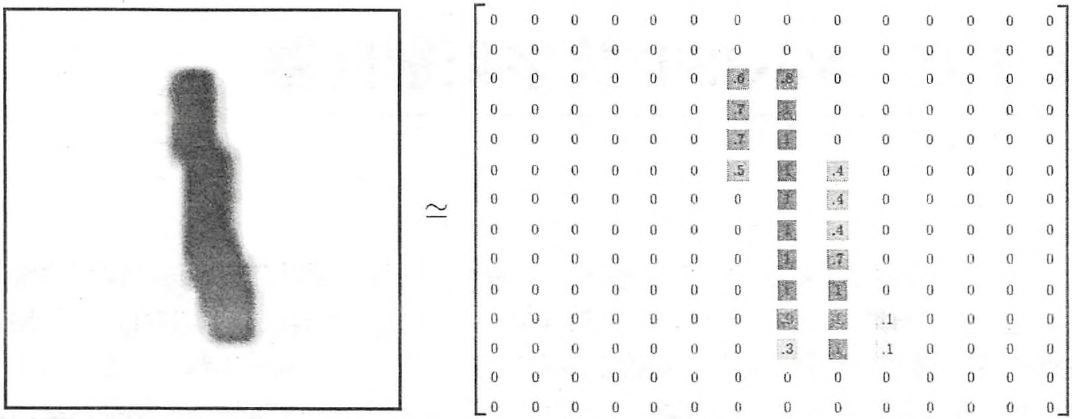
\includegraphics[width=\linewidth]{digit_example.png}
  \caption{An example of MNIST and its pixel matrix}
\end{figure}

The MNIST handwritten digits recognition is a typical task of classification. The implemented model should take a feature vector of 28x28 as input and output an integer label ranging from 0 to 9. There are many methods of classification that has been implemented on MNIST and achieved good results. In this paper, we will implement 6 methods of classfication on MNIST, observe the results of these methods and analyze the advantages and disadvantages of them. These methods are Logistic Regression, Multi-Layer Perception\,(MLP), k-Nearest Neighbor\,(KNN), Support Vector Machine\,(SVM), Convolutional neural network\,(CNN), Recurrent nerual network\,(RNN).


\section{Methodology}

\subsection{Task Definition}
Let $X = \{x_1,x_2,...\}$ be a set of feature vector of training examples and $Y = \{y_1,y_2,...\}$ be the label of training examples. Each $x_i$ is a vector of $D$ dimension. In our task, $D = 28 * 28 = 784$. Our task is to provide a $y_i$ given a new example of $x_i$ based on its feature.


\subsection{Logistic Regression}
When deep learning is not popular, logistic regression is the most common method for classification.  Logistic regression is a linear method which tries to learn a simple decision boundary for the samples. for every class $c$, it has a weight vector $W_c$ of which the number of dimensions is the same as the feature vector of a sample. we multiply $x$ with the weight vector $W_c$ to obtain a score for the class $c$. Then we use softmax to get a normalized score for each class $c$. Finally we choose the class with the highest score as the predicted label. The equation (1) shows the above process of classification.

\begin{equation}
  p(y|x) = \frac{exp(W_y\cdot x)}{\sum_{c=1}^C exp(W_c \cdot x)}
\end{equation}

During training, we minimize the cross entropy loss function over the full dataset, which is the negative log probability of the right class. 
\begin{equation}
  J(\theta) = \frac{1}{N} \sum_{i=1}^N -log(\frac{e^{f_{y_i}}}{\sum_{c=1}^C e^{f_c}} )
\end{equation}

\subsection{Support Vector Machine}
Like logistic regression, SVM also tries to find a decision boundary to classify the samples. There are many decision boundaries to split the samples, while SVM tries to find the one that has the maximum margin. The margin means the sum of the distances of two support vectors to the boundaries. The support vector is a sample which is close to the decision boundary.


\subsection{k-Nearest Neighbor}
The k-nearest neighbors algorithm (kNN) is a non-parametric method used for classification and regression. Unlike the above methods, it does not need to learn a large number of parameters to build a model. It remembers all the training samples into its memory. During prediction, It calculates the distance of the predicted sample and all the training samples. Then the model will choose k-Nearest neighbor of the predicted sample as the candidates. These neighbors will choose a label as the predicted label by voting.

\subsection{Multi-Layer Perception}
MLP is a multi-layer full-connected nonlinear neural network. At each layer $l$ , there are $I_l$ neurons with a nonlinear function, which is also called activation function. every neuron
at layer $l$ ($l > 1$) is a weighted sum of all neurons at layer $l − 1$. At training period, we also minimize the cross entropy loss function over the full dataset , like the equation (2).

\subsection{Convolutional Neural Network}
Convolutional neural network is a variant of nerual network, and it is organized by layers of neurons. Unlike MLP, there are only a few neurons conneting to each other between layers. Besides, CMM is also an unlinear model, which usually uses RELU or Tanh as an activate function to learn a more complex decision boundary. A CNN is usually formed as the following 5 modules: input layer,   convolutional layer, pooling layer, full-connected layer and softmax layer.

The convolutional layer is the most important layer in CNN. It tries to extract more abstract feature from the former layer using a filter of small size over the whole former input. Taking the image recognition as an example, the convolutional layer will make the feature deeper than the former layer to get more abstract feature. A pooling layer usually appears after the convolutional layer. It does not usually change the depth of the feature, while reduce the amount of the feature to reduce the training parameter of the whole model.
\begin{figure}[h]
  \centering
  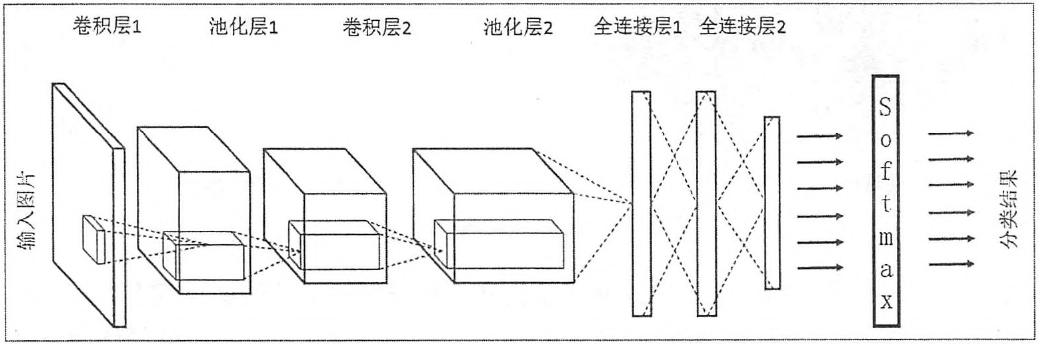
\includegraphics[width=\linewidth]{cnn.png}
  \caption{An architecture of CNN for image classification}
\end{figure}

Because of the modules of convolutional layer and pooling layer, CNN can extract more abstract features of the training data to get a more generalized model. Besides, CNN has a strong ability of Parallelism thanks to the convolutional process.  As a result, a CNN model can be trained faster than other nerual network usually. 

\subsection{Recurrent Neural Network}
RNN has a strong ability to mine the temporal information of data and model deep semantic information, which helps it to achieve some state-of-the-art performance in speech recognition, languange model, machine translation and Timing analysis. At time step $t$, RNN will output an output hidden vector $h_t$ according to the current input $x_t$. The output $h_t$ will be the input at time step $t+1$, which makes the modeling of sequential data a recurrent process.

\begin{figure}[h]
  \centering
  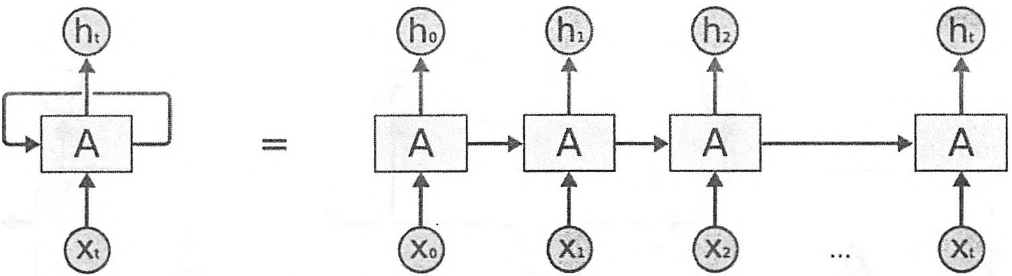
\includegraphics[width=\linewidth]{rnn.png}
  \caption{An architecture of RNN}
\end{figure}

In MNIST task, we will treat each image pixel featrue vector as a sequential data of length $D$. It will be fed to a RNN to get the final hidden state. We will use the final hidden state vector for classification.

\begin{table*}
  \caption{Overall Performance}
  \label{tab:commands}
  \begin{tabular}{1c11111}
    \toprule
    Model &epoch 1& epoch 3 & epoch 5& epoch 7& epoch 10& epoch 20\\
    \midrule
    Logistic Regression &.888& .901 & .904& .904& .904& .911\\
    SVM &.258& .373 & .497& .491& .516& .707\\
    KNN &.962& .962 & .962& .962& .962& .962\\
    MLP &.891&.903 & .902& .897& .902& .903\\
    CNN &{\bfseries .989} & {\bfseries .992} & {\bfseries .993}& {\bfseries .996}& {\bfseries .981}& {\bfseries .993}\\
    RNN &.952& .973 & .981& .973& .976& .959\\
    \bottomrule
  \end{tabular}
\end{table*}

\section{Experiments}

\subsection{Dataset}
We use the official MNIST dataset as our dataset. It has a training set of 60,000 examples, and a test set of 10,000 examples. Every example of MNIST datasets is a photo of handwritten number ranging from 0 to 9. The size of an example is 28x28, and every example digit will be located in the center of an image. 



\subsection{Our Models}
As described in 2, We will implement 6 models into MNIST recognition task to test their performance. The details of the implement ion of the above models is as below:

\textbf{Logistic Regression}: As introduced in 2.2, we use a weight matrix $W_c$ to calculate the score of every class and use softmax to normalize the score.


\textbf{Support Vector Machine}: We use the Gaussian radial basis function kernal as the kernal function in our implemention.


\textbf{k-Nearest Neighbor}: We choose the odd number ranging from 1 to 30 to observe the effect of different k for our model.


\textbf{Multi-Layer Perception}: We will use a MLP architecture of 2 layer in our model. We choose RELU as our activate function.

\textbf{Convolutional Neural Network}: We will use a CNN architecture of 2 convulutional-pooling layer in our model. We choose RELU as our activate function.

\textbf{Recurrent Neural Network}: We will use a standard RNN architecture of in our model. We choose RELU as our activate function.

\subsection{Evaluation Metrics}
We use the precision as our evaluation metric for this task, which is the most common evaluation metric in classification.

\subsection{Overall Performance}
We first give the overall results and compare the six models with each other. We also compare the results in different epoch numbers to compare the time efficiency of these models. The overall results are shown in Table 1.




\begin{enumerate}
\item  
All neural network models outperform other non-neural models significantly. The improvement of neural models confirm the effectiveness of deep learning and its ability to learn more abstract features than other models. Among three neural network models, the CNN model  is better than RNN and MLP, which performs the best result on MNIST recognition task.
\item 
The result of KNN is not concerned with the iterations of training, and it can achieve comparable results with neural models. We believe the large amount of data can benefit KNN a lot and make it comparable with neural models. 

\item 
due to the similarity of architecture between MLP and Logistic Regression, the two models  achieve similar results with each other.
\end{enumerate}





\subsection{Efficiency Analysis}

Firstly, we will make an time efficiency analysis on the six models mentioned above. Among the six models, CNN can achieve a better result and get a convergence faster than any other model due to its naturally strong ability of parallelism. the training speed of RNN is slower than CNN due to its interval structure. In non-neural models, KNN model is not in need of training of parameters, and can also get a fast training speed. SVM is the slowest model among the six models.

Secondly, we will analyze the space analysis among the six models. KNN is the most space-consuming model among the six models because it need to remember every training samples and their features. And the space consumption makes KNN achieves the fastest time efficiency. In neural world, the space consumption of models depends heavily on the number of layers of neural models. The more layer a models have, The more parameter and more training time the model need. 









%%
%% The next two lines define the bibliography style to be used, and
%% the bibliography file.
\bibliographystyle{ACM-Reference-Format}
\bibliography{sample-base}


\end{document}
\endinput
%%
%% End of file `sample-sigchi.tex'.
